
\begin{figure}[t]
    \setlength{\belowcaptionskip}{-1.25em}
    \centering
    \includegraphics[width=\linewidth]{fig__intro_a.pdf}
    \caption{Observational data (in Fig.~\protect\ref{fig:intro_fig}a)  (incorrectly) shows that high \gpugrowth leads to high latency. The trend is reversed when the data is segregated by \swapmem.}
    \label{fig:intro_fig}
\end{figure}

% \begin{figure}[tp!]
%     \setlength{\belowcaptionskip}{-0.8em}
%     \centering
%     \subfloat[\gpugrowth v. Latency]
%     {\label{fig:intro_a}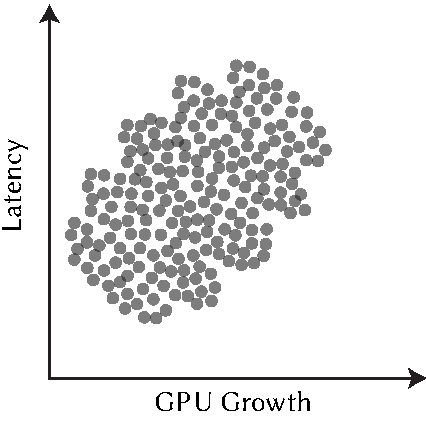
\includegraphics[width=0.45\linewidth]{fig__intro_1.pdf}}~
%     \subfloat[Observations segregated on \swapmem]
%     {\label{fig:intro_b}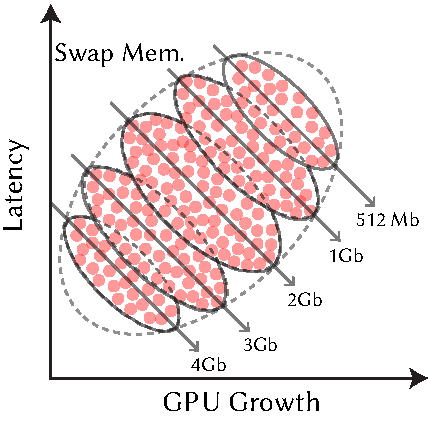
\includegraphics[width=0.45\linewidth]{fig__intro_2.pdf}}
%     \\[0.05em]
%     % \subfloat[Performance curves][Performance (Latency) curves]
%     % {\label{fig:intro_b}\includegraphics[width=0.68\linewidth]{fig__intro_b.pdf}}
%     \subfloat[][Causal Model]
%     {\label{fig:intro_c}\includegraphics[width=0.3\linewidth]{fig__intro_c.pdf}}\\[-1em]
%     \caption{\smallObservational data can sometimes lead to misleading inference. In \protectFig.~\ref{fig:intro_fig}a, the data (incorrectly) shows that high \gpugrowth leads to high latency. In \protectFig.~\ref{fig:intro_fig}b, the trend is reversed when the same data is segregated by \swapmem.}
%     \label{fig:intro_fig}
% \end{figure}
